\section{Single-Plan Verdict Calibration Ranks RL Exploitation Within the Model Ladder}\label{sec:across}

\begin{figure*}[tbp]
\centering
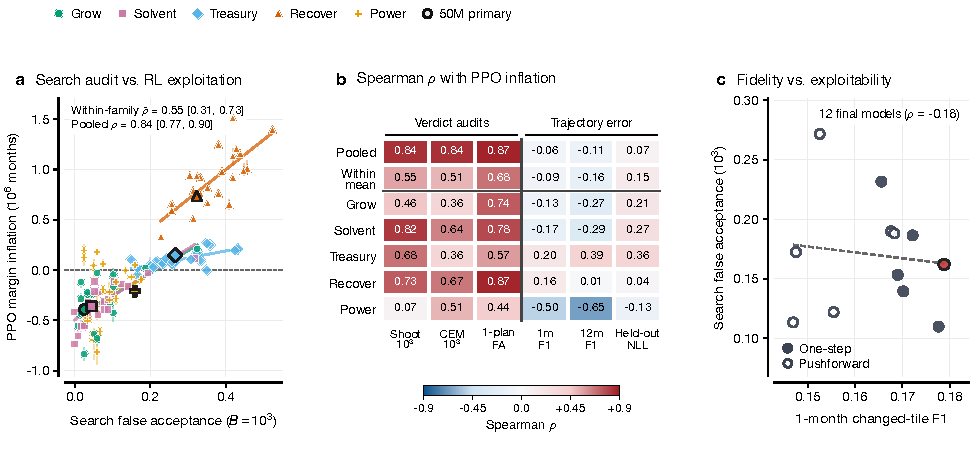
\includegraphics[width=\textwidth]{figures/fig_across.pdf}
\caption{\textbf{Task-verdict audits predict RL exploitation across \Ladder{} closely related world models, whereas standard trajectory-fidelity metrics show weak association.} \textbf{a}, Random-shooting false acceptance at $B ={}$\Bp{3} across all \AllCities{} cities vs.\ PPO continuous margin inflation after \RlMonths{} imagined months across \AcPairs{} checkpoint-by-task pairs (mean and range over three PPO seeds; dark-ringed markers denote primary \SizeM{} model; within-family Spearman \AcWithin{} \ci{\AcWithinCI}, pooled \AcRho{} \ci{\AcRhoCI}). \textbf{b}, Spearman correlation matrix comparing three verdict audits against three trajectory-error metrics. \textbf{c}, One-month changed-tile F1 vs.\ mean \Bp{3} false acceptance across the \LadFinals{} final models (\ParamsFifteen{}M, \ParamsFifty{}M, \ParamsHundred{}M; filled markers denote one-step models and hollow markers pushforward models; $\rho ={}$\AcFidFOneCkptFinalsRho{} \ci{\AcFidFOneCkptFinalsRhoCI}; \CILevel{} per cent checkpoint-cluster bootstraps).}
\label{fig:across}
\end{figure*}

Can an inexpensive offline audit rank candidate world models within a model family by how severely PPO will exploit them before policy training begins? Across our \AcClusters{} related ConvNeXt U-Net checkpoints and five task families (\AcPairs{} checkpoint-by-task observations, rather than \AcPairs{} independent architectures), we compare each checkpoint's offline task-verdict false acceptance across all \AllCities{} cities against downstream PPO exploitation after \RlMonths{} imagined steps. We track RL exploitation via PPO continuous margin inflation (imagined minus oracle margin on open-loop logs, normalised by behaviour-mix spread over three PPO seeds) and PPO pass-rate optimism (Appendix~\ref{app:acrossmore}).

Within individual task families across the \AcClusters{} checkpoints, \Bp{3} random-shooting false acceptance ranks PPO margin inflation at mean Spearman \AcWithin{} \ci{\AcWithinCI} (per-family splits and pass-rate optimism correlations appear in Appendix~\ref{app:acrossmore}). Pooled across all \AcPairs{} pairs, Spearman correlation reaches \AcRho{} \ci{\AcRhoCI} against margin inflation and \AcGapRho{} \ci{\AcGapRhoCI} against pass-rate optimism (Figure~\ref{fig:across}a; Pearson \AcPearson{} \ci{\AcPearsonCI}). Because baseline exploitability varies across task families, between-family offsets alone generate a checkpoint-permutation null median of \AcPermMid{} (\PermPct{}th percentile \AcPermHi{}), which \AcRho{} exceeds. Adaptive CEM at $B ={}$\Bp{3} across \AcAdSetName{} (\AcAdPairs{} pairs) performs similarly at \AcAdWithin{} \ci{\AcAdWithinCI} within family and \AcAdRho{} \ci{\AcAdRhoCI} pooled.

Even active search is not required within this ladder. \emph{Single-plan verdict calibration} scores one fixed logged plan per starting instance across all \AllCities{} cities (\AllInstances{} trajectories total). This audit achieves Spearman \AcEOneWithin{} \ci{\AcEOneWithinCI} within task family and \AcEOneRho{} \ci{\AcEOneRhoCI} pooled against PPO margin inflation (lineage-clustered intervals and pass-rate correlations in Appendix~\ref{app:acrossmore}). \AcECompWords{} Because that logged plan is identical across checkpoints on \AcBOneSameN{} of \AcBOneN{} instances, ground-truth engine replays are amortised once across all candidate models. Appending the \ExtTrEpochs-epoch extended-training checkpoint (\ExtTrOosCkpts{} checkpoints, \ExtTrOosPairs{} pairs; Appendix~\ref{app:extended}) preserves this ranking as spatial rollouts turn pessimistic, yielding \ExtTrOosBOneWithin{} \ci{\ExtTrOosBOneWithinCI} within-family and \ExtTrOosBOneRho{} \ci{\ExtTrOosBOneRhoCI} pooled correlation. Pairing single-plan false acceptance with single-plan false rejection (\ExtTrRandOneAllFalseRej{} at \ExtTrEpochs{} epochs vs.\ \ExtTrMainRandOneAllFalseRej{} at two epochs) flags pessimistic collapse alongside optimistic exploitation.

Standard trajectory-fidelity metrics, by contrast, show weak association with \Bp{3} random-shooting false acceptance within this \AcClusters-checkpoint ladder (Figure~\ref{fig:across}b,c). One-month structural F1 spans a narrow band (\LadFOneMin{}--\LadFOneMax{}) across the \LadFinals{} final checkpoints, comparable to single-model uncertainty \ci{\TestMainFOneCI}, which limits checkpoint-level statistical power to \AcFidPowerCkpt{} for $|\rho| = \AcFidPowerCkptRho{}$ (Appendix~\ref{app:acrossmore}). Within that band, one-month F1 correlates with \Bp{3} false acceptance at \AcFidFOneRho{} \ci{\AcFidFOneRhoCI} across \AcFidPairs{} pairs and \AcFidFOneCkptRho{} \ci{\AcFidFOneCkptRhoCI} across checkpoints, with pushforward models frequently incurring higher false acceptance than their one-step parents. Twelve-month tile F1 (\AcFidFTwelveRho{}), treasury error (\AcFidFundsRho{}), population error (\AcFidPopRho{}), held-out log-likelihood (\AcFidLikRho{}), and continuous logged-margin correlation (\AcFidDecRho{}) show similarly weak associations. Extending fidelity evaluation to month \Horizon{} across all \AcHorAllCkpts{} checkpoints (Table~\ref{tab:horizon}) likewise keeps pooled Spearman correlations within \AcHorRhoMin{} to \AcHorRhoMax{} (Appendix~\ref{app:acrossmore}). Given low checkpoint-level power over tightly clustered runs, this weak association does not prove trajectory accuracy uninformative across broader quality regimes or architectures. Among closely related checkpoints that clear shared short-horizon gates, however, residual trajectory-error differences poorly reflect task-specific boundary errors (\AcFidShareBetween{} per cent of exploitability variance sits across task predicates; \citealp{lambert2020objective}) that verdict calibration directly probes.
